\documentclass[journal,12pt,twocolumn]{article}
\usepackage[a4paper, total={6in, 8in}, margin = 0.75in]{geometry}
\usepackage{setspace}
\usepackage{gensymb}
\usepackage{caption}
%\usepackage{multirow}
%\usepackage{multicolumn}
%\usepackage{subcaption}
%\doublespacing
\singlespacing
\usepackage{csvsimple}
\usepackage{amsmath}
\usepackage{multicol}
%\usepackage{enumerate}
\usepackage{amssymb}
\usepackage{graphicx}
\graphicspath{{figs/}}
\usepackage{newfloat}
%\usepackage{syntax}
\usepackage{listings}
%\usepackage{iithtlc}
\usepackage{color}
\usepackage{tikz}
\usetikzlibrary{shapes,arrows}



%\usepackage{graphicx}
%\usepackage{amssymb}
%\usepackage{relsize}
%\usepackage[cmex10]{amsmath}
%\usepackage{mathtools}
%\usepackage{amsthm}
%\interdisplaylinepenalty=2500
%\savesymbol{iint}
%\usepackage{txfonts}
%\restoresymbol{TXF}{iint}
%\usepackage{wasysym}
\usepackage{amsthm}
\usepackage{mathrsfs}
\usepackage{txfonts}
\usepackage{stfloats}
\usepackage{cite}
\usepackage{cases}
\usepackage{mathtools}
\usepackage{caption}
\usepackage{enumerate}	
\usepackage{enumitem}
\usepackage{amsmath}
%\usepackage{xtab}
\usepackage{longtable}
\usepackage{multirow}
%\usepackage{algorithm}
%\usepackage{algpseudocode}
\usepackage{enumitem}
\usepackage{mathtools}
\usepackage{hyperref}
%\usepackage[framemethod=tikz]{mdframed}
\usepackage{listings}
    %\usepackage[latin1]{inputenc}                                 %%
    \usepackage{color}                                            %%
    \usepackage{array}                                            %%
    \usepackage{longtable}                                        %%
    \usepackage{calc}                                             %%
    \usepackage{multirow}                                         %%
    \usepackage{hhline}                                           %%
    \usepackage{ifthen}                                           %%
  %optionally (for landscape tables embedded in another document): %%
    \usepackage{lscape}     


\usepackage{url}
\def\UrlBreaks{\do\/\do-}


%\usepackage{stmaryrd}


%\usepackage{wasysym}
%\newcounter{MYtempeqncnt}
\DeclareMathOperator*{\Res}{Res}
%\renewcommand{\baselinestretch}{2}
\renewcommand\thesection{\arabic{section}}
\renewcommand\thesubsection{\thesection.\arabic{subsection}}
\renewcommand\thesubsubsection{\thesubsection.\arabic{subsubsection}}

\renewcommand\thesectiondis{\arabic{section}}
\renewcommand\thesubsectiondis{\thesectiondis.\arabic{subsection}}
\renewcommand\thesubsubsectiondis{\thesubsectiondis.\arabic{subsubsection}}

% correct bad hyphenation here
\hyphenation{op-tical net-works semi-conduc-tor}

%\lstset{
%language=C,
%frame=single, 
%breaklines=true
%}

%\lstset{
	%%basicstyle=\small\ttfamily\bfseries,
	%%numberstyle=\small\ttfamily,
	%language=Octave,
	%backgroundcolor=\color{white},
	%%frame=single,
	%%keywordstyle=\bfseries,
	%%breaklines=true,
	%%showstringspaces=false,
	%%xleftmargin=-10mm,
	%%aboveskip=-1mm,
	%%belowskip=0mm
%}

%\surroundwithmdframed[width=\columnwidth]{lstlisting}
\def\inputGnumericTable{}                                 %%
\lstset{
%language=C,
frame=single, 
breaklines=true,
columns=fullflexible
}
 

\begin{document}
%
\tikzstyle{block} = [rectangle, draw,
    text width=3em, text centered, minimum height=3em]
\tikzstyle{sum} = [draw, circle, node distance=3cm]
\tikzstyle{input} = [coordinate]
\tikzstyle{output} = [coordinate]
\tikzstyle{pinstyle} = [pin edge={to-,thin,black}]

\theoremstyle{definition}
\newtheorem{theorem}{Theorem}[section]
\newtheorem{problem}{Problem}
\newtheorem{proposition}{Proposition}[section]
\newtheorem{lemma}{Lemma}[section]
\newtheorem{corollary}[theorem]{Corollary}
\newtheorem{example}{Example}[section]
\newtheorem{definition}{Definition}[section]
%\newtheorem{algorithm}{Algorithm}[section]
%\newtheorem{cor}{Corollary}
\newcommand{\BEQA}{\begin{eqnarray}}
\newcommand{\EEQA}{\end{eqnarray}}
\newcommand{\define}{\stackrel{\triangle}{=}}
\bibliographystyle{IEEEtran}
%\bibliographystyle{ieeetr}
\providecommand{\nCr}[2]{\,^{#1}C_{#2}} % nCr
\providecommand{\nPr}[2]{\,^{#1}P_{#2}} % nPr
\providecommand{\mbf}{\mathbf}
\providecommand{\pr}[1]{\ensuremath{\Pr\left(#1\right)}}
\providecommand{\qfunc}[1]{\ensuremath{Q\left(#1\right)}}
\providecommand{\sbrak}[1]{\ensuremath{{}\left[#1\right]}}
\providecommand{\lsbrak}[1]{\ensuremath{{}\left[#1\right.}}
\providecommand{\rsbrak}[1]{\ensuremath{{}\left.#1\right]}}
\providecommand{\brak}[1]{\ensuremath{\left(#1\right)}}
\providecommand{\lbrak}[1]{\ensuremath{\left(#1\right.}}
\providecommand{\rbrak}[1]{\ensuremath{\left.#1\right)}}
\providecommand{\cbrak}[1]{\ensuremath{\left\{#1\right\}}}
\providecommand{\lcbrak}[1]{\ensuremath{\left\{#1\right.}}
\providecommand{\rcbrak}[1]{\ensuremath{\left.#1\right\}}}
\theoremstyle{remark}
\newtheorem{rem}{Remark}
\newcommand{\sgn}{\mathop{\mathrm{sgn}}}
\providecommand{\abs}[1]{\left\vert#1\right\vert}
\providecommand{\res}[1]{\Res\displaylimits_{#1}} 
\providecommand{\norm}[1]{\left\Vert#1\right\Vert}
\providecommand{\mtx}[1]{\mathbf{#1}}
\providecommand{\mean}[1]{E\left[ #1 \right]}
\providecommand{\fourier}{\overset{\mathcal{F}}{ \rightleftharpoons}}
%\providecommand{\hilbert}{\overset{\mathcal{H}}{ \rightleftharpoons}}
\providecommand{\system}{\overset{\mathcal{H}}{ \longleftrightarrow}}
	%\newcommand{\solution}[2]{\textbf{Solution:}{#1}}
\newcommand{\solution}{\noindent \textbf{Solution: }}
\newcommand{\myvec}[1]{\ensuremath{\begin{pmatrix}#1\end{pmatrix}}}
\providecommand{\dec}[2]{\ensuremath{\overset{#1}{\underset{#2}{\gtrless}}}}
\DeclarePairedDelimiter{\ceil}{\lceil}{\rceil}
%\numberwithin{equation}{section}
%\numberwithin{problem}{subsection}
%\numberwithin{definition}{subsection}
\makeatletter
\@addtoreset{figure}{section}
\makeatother
\let\StandardTheFigure\thefigure
%\renewcommand{\thefigure}{\theproblem.\arabic{figure}}
\renewcommand{\thefigure}{\thesection}
%\numberwithin{figure}{subsection}
%\numberwithin{equation}{subsection}
%\numberwithin{equation}{section}
%\numberwithin{equation}{problem}
%\numberwithin{problem}{subsection}
\numberwithin{problem}{section}
%%\numberwithin{definition}{subsection}
%\makeatletter
%\@addtoreset{figure}{problem}
%\makeatother
\makeatletter
\@addtoreset{table}{section}
\makeatother
\let\StandardTheFigure\thefigure
\let\StandardTheTable\thetable
\let\vec\mathbf
\numberwithin{equation}{section}
\vspace{3cm}
\title{%Convex Optimization in Python
	\logo{
	Random Numbers
	}
}
%\title{
%	\logo{Matrix Analysis through Octave}{\begin{center}\includegraphics[scale=.24]{tlc}\end{center}}{}{HAMDSP}
%}
% paper title
% can use linebreaks \\ within to get better formatting as desired
%\title{Matrix Analysis through Octave}
%
%
% author names and IEEE memberships
% note positions of commas and nonbreaking spaces ( ~ ) LaTeX will not break
% a structure at a ~ so this keeps an author's name from being broken across
% two lines.
% use \thanks{} to gain access to the first footnote area
% a separate \thanks must be used for each paragraph as LaTeX2e's \thanks
% was not built to handle multiple paragraphs
%
\author{ Hema Sri Cheekatla$^{*}$% <-this % stops a space
%\thanks{* The author is with the Department
%of Electrical Engineering, Indian Institute of Technology, Hyderabad
%502285 India e-mail:  gadepall@iith.ac.in.}% <-this % stops a space
%\thanks{J. Doe and J. Doe are with Anonymous University.}% <-this % stops a space
%\thanks{Manuscript received April 19, 2005; revised January 11, 2007.}}
}
% note the % following the last \IEEEmembership and also \thanks - 
% these prevent an unwanted space from occurring between the last author name
% and the end of the author line. i.e., if you had this:
% 
% \author{....lastname \thanks{...} \thanks{...} }
%                     ^------------^------------^----Do not want these spaces!
%
% a space would be appended to the last name and could cause every name on that
% line to be shifted left slightly. This is one of those "LaTeX things". For
% instance, "\textbf{A} \textbf{B}" will typeset as "A B" not "AB". To get
% "AB" then you have to do: "\textbf{A}\textbf{B}"
% \thanks is no different in this regard, so shield the last } of each \thanks
% that ends a line with a % and do not let a space in before the next \thanks.
% Spaces after \IEEEmembership other than the last one are OK (and needed) as
% you are supposed to have spaces between the names. For what it is worth,
% this is a minor point as most people would not even notice if the said evil
% space somehow managed to creep in.
% The paper headers
%\markboth{Journal of \LaTeX\ Class Files,~Vol.~6, No.~1, January~2007}%
%{Shell \MakeLowercase{\textit{et al.}}: Bare Demo of IEEEtran.cls for Journals}
% The only time the second header will appear is for the odd numbered pages
% after the title page when using the twoside option.
% 
% *** Note that you probably will NOT want to include the author's ***
% *** name in the headers of peer review papers.                   ***
% You can use \ifCLASSOPTIONpeerreview for conditional compilation here if
% you desire.
% If you want to put a publisher's ID mark on the page you can do it like
% this:
%\IEEEpubid{0000--0000/00\$00.00~\copyright~2007 IEEE}
% Remember, if you use this you must call \IEEEpubidadjcol in the second
% column for its text to clear the IEEEpubid mark.
% make the title area
\maketitle
\tableofcontents
\bigskip
\renewcommand{\thefigure}{\theenumi}
\renewcommand{\thetable}{\theenumi}
\begin{abstract}
This manual provides a simple introduction to the generation of random numbers
\end{abstract}
%%
\section{Uniform Random Numbers}
Let $U$ be a uniform random variable between 0 and 1.
\begin{enumerate}[label=\thesection.\arabic*
,ref=\thesection.\theenumi]
\item Generate $10^6$ samples of U using a C program and save into a file called uni.dat.
\\
\solution 
Download the following files and execte the C program.
\begin{lstlisting}
wget https://github.com/Hema-Sri-Ch/AI1110-Assignments/Assignment/codes/exrand.c
wget https://github.com/Hema-Sri-Ch/AI1110-Assignments/Assignment/codes/coeffs.h
\end{lstlisting}
And run the following commands in the terminal to execute the C program files
\begin{lstlisting}
gcc -o out exrand.c coeffs.h -lm
./out
\end{lstlisting}
Then the corresponding "uni.dat" file will be created with $10^6$ samples of U.

\item
Load the uni.dat file into python and plot the empirical CDF of $U$ using the samples in uni.dat. The CDF is defined as
\begin{align}
F_{U}(x) = \pr{U \le x}
\end{align}
\\
\solution  The following code plots Fig. \ref{fig:uni_cdf} in the figs folder(Comment out or remove comments for some lines accordingly)
\begin{lstlisting}
wget https://github.com/Hema-Sri-Ch/AI1110-Assignments/Assignment/codes/cdf_plot.py
\end{lstlisting}
And execute the following command in the terminal 
\begin{lstlisting}
python3 cdf_plot.py
\end{lstlisting}
\begin{figure}[h]
	\centering
	\includegraphics[width=\columnwidth]{uni_cdf}
	\caption{The CDF of $U$}
	\label{fig:uni_cdf}
\end{figure}
%
\item
Find a  theoretical expression for $F_{U}(x)$.
\\
\solution We know that the PDF of a uniform distribution function in a particular intervel (a, b) is given by,
\begin{align}
	f(x) &= \begin{cases} \frac{1}{b-a} &,\text{ for } a \leq x \leq b \\
	0 &, otherwise\end{cases}
\end{align}
Hence, the PDF of this uniform distribution is given as follows in this particular interval of (0, 1) is given by as follows,
\begin{align}
	f(x) &= \begin{cases} 1 &,\text{ for } a \leq x \leq b \\
	0 &, otherwise\end{cases}
\end{align}

Hence, the CDF of a uniform distribution function is given as follows in a particular interval (a, b) is given by,
\begin{align}
	F_U(x) &= \int_{-\infty}^{x} f(x) \, dx \\
		&= \begin{cases} \int_{-\infty}^{x} 0 \, dx &, x < 0 \\
		\int_{0}^{x} \, dx &, 0 \leq x \leq 1 \\
		\int_{0}^{1} \, dx &, x > 1 
		\end{cases} \\
		&= \begin{cases}0 &, x<0 \\
		1[x]_{0}^{x} &, 0 \leq x \leq 1 \\
		1[x]_{0}^{1} + 0 &, x >1\end{cases} \\
	\implies F_U(x)	&= \begin{cases} 0 &, \text{ for } x < 0\\
	x &, \text{ for } 0 \leq x \leq 1 \\
	 1 &, \text{ for } x > 1\end{cases}
\end{align}

In Our case, the intervel is (0, 1). Hence the theoretical expression for $F_U(x)$ is given as follows,

\begin{align}
	F_U(x) &= \begin{cases} 0 &, \text{ for } x < 0\\
	 x &, \text{ for } 0 \leq x \leq 1 \\
	 1 &, \text{ for } x > 1\end{cases}
\end{align}

\item
The mean of $U$ is defined as
%
\begin{equation}
E\sbrak{U} = \frac{1}{N}\sum_{i=1}^{N}U_i
\end{equation}
%
and its variance as
%
\begin{equation}
\text{var}\sbrak{U} = E\sbrak{U- E\sbrak{U}}^2 
\end{equation}
Write a C program to  find the mean and variance of $U$. 
\\
\solution Download the following files and execte the C program.
\begin{lstlisting}
wget https://github.com/Hema-Sri-Ch/AI1110-Assignments/Assignment/codes/exrand.c
wget https://github.com/Hema-Sri-Ch/AI1110-Assignments/Assignment/codes/coeffs.h
\end{lstlisting}
And run the following commands in the terminal to execute the C program files
\begin{lstlisting}
gcc -o out exrand.c coeffs.h -lm
./out
\end{lstlisting}
The Mean and Variance of $U$ is written as output in the terminal.

\item Verify your result theoretically given that
\end{enumerate}
%
\begin{equation}
E\sbrak{U^k} = \int_{-\infty}^{\infty}x^kdF_{U}(x)
\end{equation}
\\
\solution
If k = 1, then E[$U^1$] is nothing but the mean of this uniform distribution,\newline
Theoretically, we have 
\begin{align}
	F_U(x) &= \begin{cases} 0 &, \text{ for } x < 0\\
	 x &, \text{ for } 0 \leq x \leq 1 \\
	 1 &, \text{ for } x > 1\end{cases}
\end{align}
Hence $dF_U(x)$ can be written as follows,
\begin{align}
	dF_U(x) &= f(x) = \begin{cases} 1 &,\text{ for } 0 \leq x \leq 1 \\
	0 &, otherwise\end{cases} \\
	\implies E[U] &= \int_{0}^{1} x \,dx \\
	&= 0.5
\end{align}
Hence our theoretical mean is 0.5, where as we got our practical mean as 0.500007, which is almost same.\newline
Hence our expression is verified for k = 1.\newline
Similarly we can consider k = 2, then we get,
\begin{align}
	E[U^2] &= \int_{0}^{1} x^2 \, dx \\
	&= 0.333333 
\end{align}
Hence our theoretical value of $E[U^2]$ is 0.333333, where we got our practical value of $E[U^2]$ as 0.333308, which is again almost same as that of theoretical value.\newline
Hence Verified.

\section{Central Limit Theorem}
%
\begin{enumerate}[label=\thesection.\arabic*
,ref=\thesection.\theenumi]
%
\item
Generate $10^6$ samples of the random variable
%
\begin{equation}
X = \sum_{i=1}^{12}U_i -6
\end{equation}
%
using a C program, where $U_i, i = 1,2,\dots, 12$ are  a set of independent uniform random variables between 0 and 1
and save in a file called gau.dat
%
\\
\solution Download the following files and execte the C program.
\begin{lstlisting}
wget https://github.com/Hema-Sri-Ch/AI1110-Assignments/Assignment/codes/exrand.c
wget https://github.com/Hema-Sri-Ch/AI1110-Assignments/Assignment/codes/coeffs.h
\end{lstlisting}
And run the following commands in the terminal to execute the C program files
\begin{lstlisting}
gcc -o out exrand.c coeffs.h -lm
./out
\end{lstlisting}
Then the corresponding "gau.dat" file will be created with $10^6$ samples of X.

\item
Load gau.dat in python and plot the empirical CDF of $X$ using the samples in gau.dat. What properties does a CDF have?
\\
\solution The following code plots Fig. \ref{fig:gauss_cdf} in the figs folder(Comment out or remove comments for some lines accordingly)
\begin{lstlisting}
wget https://github.com/Hema-Sri-Ch/AI1110-Assignments/Assignment/codes/cdf_plot.py
\end{lstlisting}
And execute the following command in the terminal 
\begin{lstlisting}
python3 cdf_plot.py
\end{lstlisting}
\begin{figure}[h]
	\centering
	\includegraphics[width=\columnwidth]{gauss_cdf}
	\caption{The CDF of $X$}
	\label{fig:gauss_cdf}
\end{figure}

To find cdf of this gaussian function, we have its pdf as,
\begin{align}
	f(x) &= \frac{1}{\sqrt{2\pi}} e^{\frac{-x^2}{2}} , -\infty < x < \infty \\
	\implies F(x) &= 1 - \pr{\vec{x} > x} \\
	&=  1 - Q(x)
\end{align}
\item
Load gau.dat in python and plot the empirical PDF of $X$ using the samples in gau.dat. The PDF of $X$ is defined as
\begin{align}
p_{X}(x) = \frac{d}{dx}F_{X}(x)
\end{align}
What properties does the PDF have?
\\
\solution The following code plots Fig. \ref{fig:gauss_pdf} in the figs folder(Comment out or remove comments for some lines accordingly)
\begin{lstlisting}
wget https://github.com/Hema-Sri-Ch/AI1110-Assignments/Assignment/codes/pdf_plot.py
\end{lstlisting}
And execute the following command in the terminal 
\begin{lstlisting}
python3 pdf_plot.py
\end{lstlisting}
\begin{figure}[h]
	\centering
	\includegraphics[width=\columnwidth]{gauss_pdf}
	\caption{The PDF of $X$}
	\label{fig:gauss_pdf}
\end{figure}

\item Find the mean and variance of $X$ by writing a C program.
\\
\solution
Download the following files and execte the C program.
\begin{lstlisting}
wget https://github.com/Hema-Sri-Ch/AI1110-Assignments/Assignment/codes/exrand.c
wget https://github.com/Hema-Sri-Ch/AI1110-Assignments/Assignment/codes/coeffs.h
\end{lstlisting}
And run the following commands in the terminal to execute the C program files
\begin{lstlisting}
gcc -o out exrand.c coeffs.h -lm
./out
\end{lstlisting}
The Mean and Variance of $X$ is written as output in the terminal.

\item Given that 
\begin{align}
p_{X}(x) = \frac{1}{\sqrt{2\pi}}\exp\brak{-\frac{x^2}{2}}, -\infty < x < \infty,
\end{align}
repeat the above exercise theoretically.
%
\\
\solution
We know that,
\begin{align}
	Mean &= E[U] = \int_{-\infty}^{\infty} x p_X(x) \, dx\\
	&= \int_{-\infty}^{\infty} x \frac{1}{\sqrt{2\pi}}exp(-\frac{x^2}{2}) \, dx
\end{align}
Since the function $x \frac{1}{\sqrt{2\pi}}exp(-\frac{x^2}{2})$ is an odd function, its integral in the interval $(-\infty, \infty)$ is zero.
Hence the Theoretical Mean is 0, whereas the practical Mean we have obtained is 0.000326 which is almost as same as that of Theoretical Mean\newline

We know that,
\begin{align}
	Varience &= E[U^2] - E[U]^2 \\
	\implies Variance &= E[U^2] \\
	Variance &= E[U^2] \\
	&= \int_{-\infty}^{\infty} x^2 p_X(x) \, dx \\
	&= \int_{-\infty}^{\infty} x^2 \frac{1}{\sqrt{2\pi}}e^{-\frac{x^2}{2}} \,dx \\
	&= \frac{2\sqrt{2}}{\sqrt{2\pi}} \int_{-\infty}^{\infty} x^2 e^{-x^2} \, dx 
\end{align}

Let $u=x$ and $v = e^{-x^2}$, then we have $\frac{dv}{dx} = -2xe^{-x^2}$. Intergration by parts for the expression 
\begin{align} 
	\int_{-\infty}^{\infty} x^2 e^{-x^2} \, dx &= -\frac{1}{2} \int_{-\infty}^{\infty} x . (-2xe^{-x^2}) \, dx \\
	&= -\frac{1}{2}uv|_{-\infty}^{\infty} + \frac{1}{2} \int_{-\infty}^{\infty} v \frac{du}{dx}  dx 
\end{align}
\begin{align}
	= -\frac{1}{2}x \int_{-\infty}^{\infty}(-2xe^{-x^2}) dx +\frac{1}{2} \int_{-\infty}^{\infty} e^{-x^2}  dx 
\end{align}
since the first term of this expression is odd fuction its value is 0. And from the gaussian distribution, we have
\begin{align}
	\int_{-\infty}^{\infty} \frac{1}{\sqrt {2\pi}} e^{-x^2/2} \, dx &= 1 \\
	\implies \int_{-\infty}^{\infty} e^{-x^2} \, dx &= \sqrt{\pi} \\
	\text{Hence, } \int_{-\infty}^{\infty} x^2 e^{-x^2} \, dx &= \frac{\sqrt{\pi}}{2} 
\end{align}

Hence the Theoretical Variance is 1, whereas the practical Varaince we have obtained is 1.000907 which is almost as same as that of the Theoretical Varaince\newline

\end{enumerate}
\section{From Uniform to Other}
\begin{enumerate}[label=\thesection.\arabic*
,ref=\thesection.\theenumi]
%
\item
Generate samples of 
%
\begin{equation}
V = -2\ln\brak{1-U}
\end{equation}
%
and plot its CDF.
\\  
\solution
Download the following files and execte the C program.
\begin{lstlisting}
wget https://github.com/Hema-Sri-Ch/AI1110-Assignments/Assignment/codes/exrand.c
wget https://github.com/Hema-Sri-Ch/AI1110-Assignments/Assignment/codes/coeffs.h
\end{lstlisting}
And run the following commands in the terminal to execute the C program files
\begin{lstlisting}
gcc -o out exrand.c coeffs.h -lm
./out
\end{lstlisting}
Then the corresponding "req.dat" file will be created with $10^6$ samples of V.
The following code plots Fig. \ref{fig:req_cdf} in the figs folder.(Comment out or remove comments for some lines accordingly)
\begin{lstlisting}
wget https://github.com/Hema-Sri-Ch/AI1110-Assignments/Assignment/codes/cdf_plot.py
\end{lstlisting}
And execute the following command in the terminal 
\begin{lstlisting}
python3 cdf_plot.py
\end{lstlisting}
\begin{figure}[h]
	\centering
	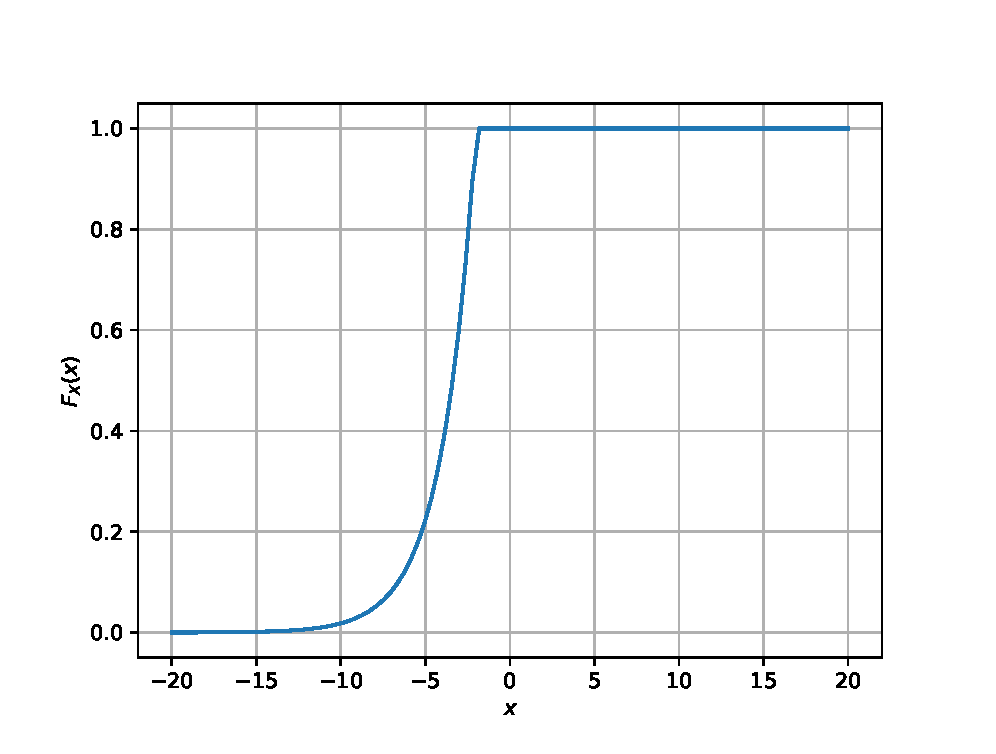
\includegraphics[width=\columnwidth]{req_cdf}
	\caption{The CDF of $V$}
	\label{fig:req_cdf}
\end{figure}
\item Find a theoretical expression for $F_V(x)$.
\\
\solution We know that,

\begin{align}
	F_V(x) &= P(V \leq x) \\
	F_V(x) &= P(-2 \ln(1-U) \leq x) \\
	F_V(x) &= P(\ln(1-U) \geq -\frac{x}{2}) \\
	F_V(x) &= P(1-U \geq e^{-\frac{x}{2}}) \\
	F_V(x) &= P(U \leq 1-e^{-\frac{x}{2}}) \\
	F_V(x) &= F_U(1-e^{-\frac{x}{2}}) \\
	\text{Hence, } F_V(x) &= \begin{cases} 0 &, 1-e^{-x/2} < 0 \\
	1-e^{-\frac{x}{2}} &, 0 \leq 1-e^{-x/2} \leq 1 \\
	1 &, 1-e^{-x/2} > 1 \end{cases}
\end{align}

From this we get,
\begin{align}
	F_V(x) &= \begin{cases} 0 &, x < 0 \\
	1 - e^{-x/2} &, x>0\end{cases}
\end{align}
%
%\item
%Generate the Rayleigh distribution from Uniform. Verify your result through graphical plots.
\end{enumerate}
\section{Triangular Distribution}
\begin{enumerate}[label=\thesection.\arabic*
,ref=\thesection.\theenumi]
%
\item
Generate
\begin{align}
	T = U_1 + U_2
\end{align}
\\
\solution Download the following files and execte the C program.
\begin{lstlisting}
wget https://github.com/Hema-Sri-Ch/AI1110-Assignments/Assignment/codes/exrand.c
wget https://github.com/Hema-Sri-Ch/AI1110-Assignments/Assignment/codes/coeffs.h
\end{lstlisting}
And run the following commands in the terminal to execute the C program files
\begin{lstlisting}
gcc -o out exrand.c coeffs.h -lm
./out
\end{lstlisting}
Then the corresponding "tri.dat" file will be created with $10^6$ samples of T.
\\
\item
Find the CDF of T
\\
\solution The following code plots Fig. \ref{fig:tri_cdf} in the figs folder(Comment out or remove the comments accordingly)
\begin{lstlisting}
wget https://github.com/Hema-Sri-Ch/AI1110-Assignments/Assignment/codes/cdf_plot.py
\end{lstlisting}
And execute the following command in the terminal 
\begin{lstlisting}
python3 cdf_plot.py
\end{lstlisting}
\begin{figure}[h]
	\centering
	\includegraphics[width=\columnwidth]{tri_cdf}
	\caption{The CDF of $T$}
	\label{fig:tri_cdf}
\end{figure}

\item
Find the PDF of T
\\
\solution The following code plots Fig. \ref{fig:tri_pdf} in the figs folder(Comment out or remove the comments accordingly)
\begin{lstlisting}
wget https://github.com/Hema-Sri-Ch/AI1110-Assignments/Assignment/codes/pdf_plot.py
\end{lstlisting}
And execute the following command in the terminal 
\begin{lstlisting}
python3 pdf_plot.py
\end{lstlisting}
\begin{figure}[h]
	\centering
	\includegraphics[width=\columnwidth]{tri_pdf}
	\caption{The PDF of $T$}
	\label{fig:tri_pdf}
\end{figure}

\item
Find the theoretical expressions for the PDF and the CDF of T
\\
\solution
We have,
\begin{align}
	T &= U_1 + U_2 
\end{align}
Where $U_1$ and $U_2$ are independent random variables in the interval (0, 1). Hence it is clear that the random numbers of T lies between 0 and 2\\
Now the PDF of T is given as follows,
\begin{align}
	p_T(t) &= \int_{-\infty}^{\infty} f_X(x)f_Y(t-x) \, dx \\ 
\end{align}
We have, $p_T(t) = 0$ for $t < 0$ and for $t > 2$. Hence we need to find $p_T(t)$ in the interval (0, 2).\newline
for $0 < t < 1 $, $f_X(x)f_Y(t-x) = 1$ for some x and 0 for else. In order to have $f_Y(t-x) = 1$, $t-x \geq 0$ which imples $x \leq t$. Hence,
\begin{align}
	p_T(t) &= \int_{0}^{1} f_X(x)f_Y(t-x) \, dx \\
	&= \int_{0}^{t} 1 \,dx \\
	&= t
\end{align}
for $1 < t < 2$, $f_X(x)f_Y(t-x) = 1$ for some x and 0 for else. In order to have $f_Y(t-x) = 1$, $t-x \leq 1$ which imples $x \geq t-1$. Hence,
\begin{align}
	p_T(t) &= \int_{0}^{1} f_X(x)f_Y(t-x) \, dx \\
	&= \int_{t-1}^{1} 1 \,dx \\
	&= 2 - t
\end{align}
Hence the PDF of T is given s follows,
\begin{align}
	p_T(t) &= \begin{cases} 0 &, 0 < t \\
	t &, 0 < t \leq 1 \\
	2 - t &, 1 < t \leq 2 \\
	0 &, t > 2 \end{cases} 
\end{align}
The CDF of T is given as follows,
\begin{align}
	F_T(x) &= \int_{-\infty}^{x} p_T(t) \, dt \\
\end{align}
For $t < 0$ ;
\begin{align}
	F_T(x) &= \int_{-\infty}^{x} p_T(t) \, dt \\
	&= \int_{-\infty}^{x} 0 \, dt \\
	&= 0
\end{align}
For $0 < t < 1$,
\begin{align}
	F_T(x) &= \int_{-\infty}^{x} p_T(t) \, dt \\
	&= \int_{-\infty}^{0} 0 \, dt  + \int_{0}^{x} t \, dt\\
	&= 0 + \frac{t^2}{2}|_{0}^{x} \\
	&= \frac{x^2}{2}
\end{align}
For $1 < t < 2$,
\begin{align}
	F_T(x) &= \int_{-\infty}^{x} p_T(t) \, dt \\
	&= \int_{-\infty}^{0} 0 \, dt  + \int_{0}^{1} t \, dt + \int_{1}^{x} 2-t \, dt\\
	&= 0 + \frac{t^2}{2}|_{0}^{1} + [2t - t^2/2]_{1}^{x}\\
	&= -\frac{x^2}{2} + 2x - 1
\end{align}
For $t > 2$
\begin{align}
	F_T(x) &= \int_{-\infty}^{x} p_T(t) \, dt \\
	&= \int_{0}^{1} t \, dt + \int_{1}^{2} 2-t \, dt \\
	&= 0 + \frac{t^2}{2}|_{0}^{1} + [2t - t^2/2]_{1}^{2}\\
	&= 1
\end{align}
Hence the CDF of T is given s follows,
\begin{align}
	F_T(x) &= \begin{cases} 0 &, 0 < x \\
	\frac{x^2}{2} &, 0 < x \leq 1 \\
	-\frac{x^2}{2} + 2x - 1 &, 1 < x \leq 2 \\
	1 &, x > 2 \end{cases} 
\end{align}

\item
Verify your results through a plot
\\
\solution
The figs \ref{fig:tri_cdf} and \ref{fig:tri_pdf} shows the required verification
\begin{lstlisting}
wget https://github.com/Hema-Sri-Ch/AI1110-Assignments/Assignment/codes/pdf_plot.py
wget https://github.com/Hema-Sri-Ch/AI1110-Assignments/Assignment/codes/pdf_plot.py
python3 pdf_plot.py
python3 cdf_plot.py
\end{lstlisting}
\end{enumerate}
\end{document}
